\documentclass[10pt,a4paper]{article}

% ------------------------------------------------------------------ Paquetes
\usepackage[utf8]{inputenc}
\usepackage[T1]{fontenc}
\usepackage[spanish,es-tabla,es-nodecimaldot]{babel}
\usepackage[a4paper,margin=2cm]{geometry} % ancho de texto = 17 cm (= ancho de las figuras)
\usepackage{graphicx}
\usepackage{booktabs}
\usepackage{float}
\usepackage{amsmath}
\usepackage{newtxtext,newtxmath}          % Times: coincide con la fuente de las figuras
\usepackage[font=small,labelfont=bf,skip=4pt]{caption}
\usepackage[compact]{titlesec}
\usepackage{enumitem}
\usepackage[super]{cite}                  % citas numéricas en superíndice, estilo artículo
\usepackage[hidelinks]{hyperref}

\titlespacing*{\section}{0pt}{8pt}{3pt}
\setlength{\parskip}{3pt}
\setlength{\parindent}{0pt}
\setlist{nosep,leftmargin=*}
\setlength{\textfloatsep}{8pt}
\setlength{\floatsep}{6pt}
\setlength{\intextsep}{6pt}

\graphicspath{{figuras/}}
% Generado automáticamente por generar_figuras.py; no editar a mano.
\newcommand{\Nmuestras}{27\,129}
\newcommand{\tIni}{90.1}
\newcommand{\tFin}{879.3}
\newcommand{\duracion}{789.2}
\newcommand{\xMin}{-1.34}
\newcommand{\xMax}{13.69}
\newcommand{\yMin}{-3.88}
\newcommand{\yMax}{11.22}
\newcommand{\dtMedio}{29.1}
\newcommand{\dtMediana}{25}
\newcommand{\dtMin}{16}
\newcommand{\dtMax}{236}
\newcommand{\dtStd}{14.0}
\newcommand{\fMuestreo}{34.4}
\newcommand{\nHuecos}{104}
\newcommand{\pasoMedio}{8.8}
\newcommand{\pasoMax}{71.4}
\newcommand{\distancia}{237.9}
\newcommand{\vGlobal}{0.301}
\newcommand{\desplNeto}{3.03}
\newcommand{\desplPct}{1.27}
\newcommand{\vMedia}{0.367}
\newcommand{\vMax}{3.47}
\newcommand{\vMin}{0.0085}
\newcommand{\vPnoventaycinco}{1.05}
\newcommand{\tvMax}{529.6}
\newcommand{\vLenta}{0.6}
\newcommand{\wMedia}{0.047}
\newcommand{\wAbsMedia}{2.74}
\newcommand{\wAbsMediana}{1.85}
\newcommand{\wMax}{39.27}
\newcommand{\wSuaveAbsMedia}{0.25}
\newcommand{\giroNeto}{33.8}
\newcommand{\vueltas}{5.4}
\newcommand{\corrVW}{-0.147}
\newcommand{\aLatMax}{7.70}
\newcommand{\aAbsMedia}{1.09}
\newcommand{\aPuno}{-4.40}
\newcommand{\aPnoventaynueve}{4.56}
\newcommand{\nRepetidos}{10}
\newcommand{\xCero}{13.689}
\newcommand{\yCero}{-1.035}
\newcommand{\thetaCero}{3.034}
\newcommand{\thetaCeroGrados}{173.8}
\newcommand{\sigmaV}{0.00367}
\newcommand{\sigmaW}{0.0274}
\newcommand{\Nruns}{100}
\newcommand{\cUnoFinal}{$1.2\times10^{-13}$}
\newcommand{\cUnoMax}{$3.9\times10^{-13}$}
\newcommand{\cUnoRmse}{$1.9\times10^{-13}$}
\newcommand{\cDosFinal}{0.0164}
\newcommand{\cDosFinalStd}{0.0101}
\newcommand{\cDosMax}{0.0228}
\newcommand{\cDosMaxStd}{0.0083}
\newcommand{\cDosRmse}{0.0127}
\newcommand{\cDosRmseStd}{0.0051}
\newcommand{\cDosPct}{0.0069}
\newcommand{\cTresFinal}{1.5440}
\newcommand{\cTresFinalStd}{1.0289}
\newcommand{\cTresMax}{1.8592}
\newcommand{\cTresMaxStd}{0.8693}
\newcommand{\cTresRmse}{0.7832}
\newcommand{\cTresRmseStd}{0.2639}
\newcommand{\cTresPct}{0.649}
\newcommand{\ratioErr}{94}
   % valores numéricos generados por generar_figuras.py

% ------------------------------------------------------------------ Documento
\begin{document}

\begin{center}
  {\Large\bfseries Odometría de una plataforma diferencial a partir de su trayectoria}\\[4pt]
  {\normalsize Jose Marcial Galván}\\[1pt]
  {\small Sistemas Robóticos Autónomos -- ULPGC}
\end{center}

\section{Datos de partida}

El fichero \texttt{Path\_SRA2526.txt} contiene \Nmuestras{} muestras $(x_k, y_k, t_k)$ de la
trayectoria de un robot diferencial entre $t=\tIni$ y $t=\tFin$~s (\duracion~s). Se carga con
\texttt{numpy.loadtxt}\cite{gfg} como un array estructurado con campos \texttt{x}, \texttt{y},
\texttt{t}\cite{numpy}, y las figuras se generan con Matplotlib\cite{matplotlib}. Las coordenadas
tienen resolución de 1~mm y el robot se mueve en un área de unos $15\times15$~m
($x\in[\xMin,\xMax]$, $y\in[\yMin,\yMax]$~m). El muestreo \emph{no es uniforme}, por lo que todos
los cálculos usan el $\Delta t_k = t_{k+1}-t_k$ real de cada intervalo.

\section{Apartado a): velocidades lineal y angular}

En una plataforma diferencial sin deslizamiento lateral la velocidad es siempre tangente a la
trayectoria\cite{upv}. Por ello, la velocidad lineal es la distancia entre dos muestras dividida por
su $\Delta t$, y la orientación es la dirección del desplazamiento. La velocidad angular es la
variación de esa orientación por unidad de tiempo\cite{wiki}, previamente desenrollada para evitar
saltos de $2\pi$:
\begin{equation*}
  v_k = \frac{\sqrt{\Delta x_k^2+\Delta y_k^2}}{\Delta t_k},\qquad
  \theta_k = \operatorname{atan2}(\Delta y_k,\Delta x_k),\qquad
  \omega_k = \frac{\theta_{k+1}-\theta_k}{\Delta t_{k+1}} .
\end{equation*}

\begin{figure}[!htb]
  \centering
  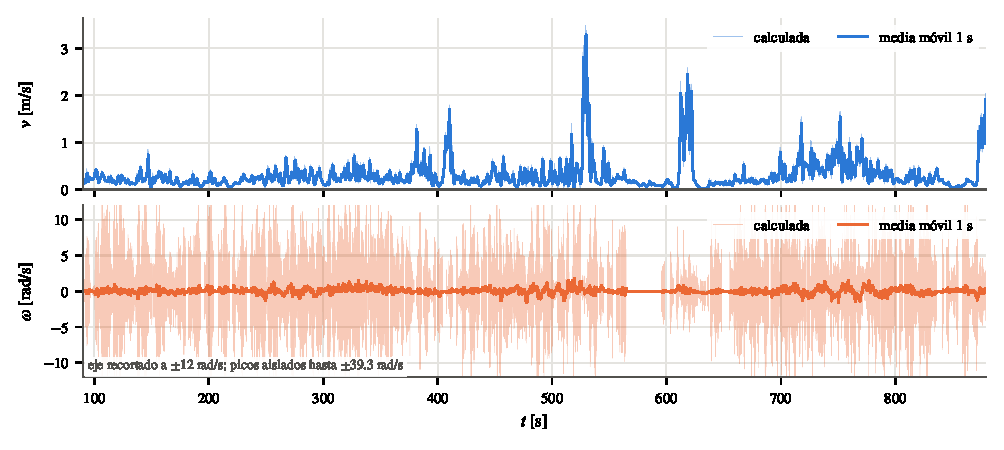
\includegraphics[width=\textwidth]{velocidades.pdf}
  \caption{Velocidades lineal $v$ (arriba) y angular $\omega$ (abajo) calculadas a partir de la
  trayectoria. En trazo fino, el valor de cada intervalo; en trazo grueso, su media móvil de 1~s.}
  \label{fig:vel}
\end{figure}

La velocidad lineal (fig.~\ref{fig:vel}) es casi siempre baja, con varios tramos rápidos en
rectas largas. La velocidad angular presenta un ruido muy alto, con picos de $\pm\wMax$~rad/s
($=\pm\pi/0.08$, un giro aparente de $180^\circ$ en 80~ms). No son giros reales sino un efecto de
la \textbf{cuantificación de 1~mm}: con pasos medios de \pasoMedio~mm, un error de 1~mm en la
posición ya cambia la dirección del segmento en $\sim$0.1~rad, y al dividir por
$\Delta t\approx25$~ms se convierte en varios rad/s. Promediando en 1~s, $\overline{|\omega|}$
baja de \wAbsMedia{} a \wSuaveAbsMedia~rad/s, valor más próximo al que mediría un giróscopo real.

\section{Apartado b): información útil para un sistema robótico}

La tabla~\ref{tab:estadisticos} reúne los valores medios, medianos, mínimos y máximos de las
magnitudes que caracterizan el movimiento del robot y el sensor que lo registró. De ellos se
extrae lo siguiente:


\begin{itemize}
  \item \textbf{Muestreo.} El periodo medio es de \dtMedio~ms ($\approx$\fMuestreo~Hz), pero varía
    entre \dtMin{} y \dtMax~ms y hay \nHuecos{} intervalos de más de 100~ms
    (fig.~\ref{fig:analisis}b). Nunca hay dos muestras iguales (paso mínimo de 1~mm) y los
    intervalos largos aparecen con el robot casi parado: la velocidad media en ellos es 0.06~m/s,
    frente a 0.46~m/s cuando $\Delta t<30$~ms. Esto sugiere que el registro solo guarda una muestra
    cuando la posición cambia, y explica que la media por muestra de $v$ (\vMedia~m/s) supere a la
    media temporal real (\distancia~m en \duracion~s, es decir, \vGlobal~m/s).
  \item \textbf{Velocidad lineal.} La mediana (0.26~m/s) muestra que el robot trabaja casi siempre
    despacio, sobre todo en las zonas con bucles (fig.~\ref{fig:analisis}a). El máximo,
    \vMax~m/s en $t\approx\tvMax$~s, aparece en las rectas diagonales y fija el límite que deben
    soportar motores y controlador. El mínimo (0.009~m/s) indica que no llega a detenerse por
    completo. La correlación entre $v$ y $|\omega|$ es de $\corrVW$: el robot frena ligeramente al girar.
  \end{itemize}

\begin{table}[H]
  \centering\small
  \caption{Estadísticos de las magnitudes obtenidas a partir de la trayectoria.}
  \label{tab:estadisticos}
  \begin{tabular}{@{}lrrrr@{}}
    \toprule
    Magnitud & Media & Mediana & Mínimo & Máximo \\
    \midrule
    \csname @@input\endcsname tabla_estadisticos.tex
    \bottomrule
  \end{tabular}
\end{table}

\begin{itemize}
  \item \textbf{Velocidad angular.} La media de $\omega$ es positiva: el giro neto acumulado es de
    \giroNeto~rad ($\approx$\vueltas{} vueltas en sentido antihorario). Una vez filtrada, $\omega$
    queda entre $-1.58$ y $1.77$~rad/s. Entre $t\approx570$ y 600~s el robot avanza paralelo al eje
    $y$, $\Delta x=0$ y $\omega=0$ exactamente en el 93\,\% de las muestras, lo que confirma que el
    ruido de $\omega$ procede de la cuantificación.
  \item \textbf{Aceleraciones.} Son las magnitudes más ruidosas, porque se obtienen derivando dos
    veces posiciones cuantificadas: los extremos de $\pm13$~m/s$^2$ y la aceleración lateral máxima
    de \aLatMax~m/s$^2$ están sobrestimados. Para dimensionar par motor o riesgo de derrape habría
    que filtrarlas primero.
  \item \textbf{Ruta.} Termina a \desplNeto~m del inicio (\desplPct\,\% del recorrido), así que es
    casi cerrada, y pasa \nRepetidos{} veces por puntos ya visitados.
\end{itemize}

\begin{figure}[!htb]
  \centering
  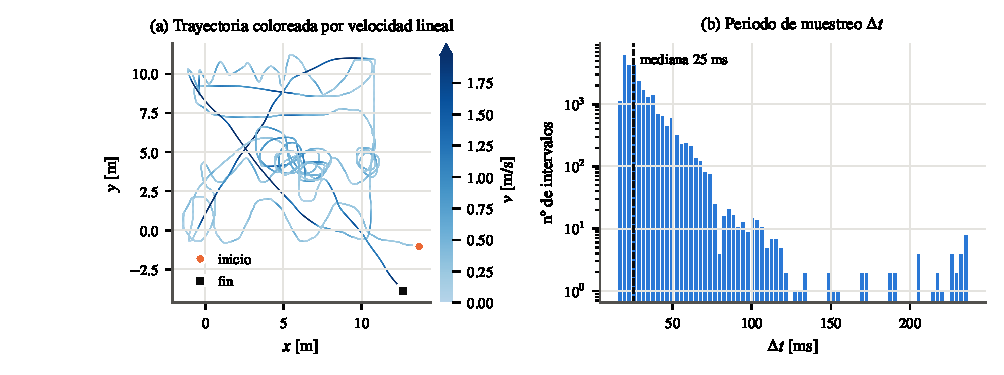
\includegraphics[width=\textwidth]{analisis.pdf}
  \caption{(a) Trayectoria con la velocidad lineal en color. (b) Histograma del periodo de muestreo
  (escala logarítmica).}
  \label{fig:analisis}
\end{figure}

\section{Apartado c): reconstrucción de la trayectoria}

Partiendo de la pose inicial conocida, $(x_0,y_0,\theta_0)=(\xCero, \yCero, \thetaCero\text{ rad})$
($\theta_0=\thetaCeroGrados^\circ$, dirección del primer segmento), se integra el modelo cinemático
diferencial\cite{upv} con el método de Euler:
\begin{equation*}
  \theta_{k+1} = \theta_k + \omega_k\,\Delta t_{k+1},\qquad
  x_{k+1} = x_k + v_k\,\Delta t_k\cos\theta_k,\qquad
  y_{k+1} = y_k + v_k\,\Delta t_k\sin\theta_k .
\end{equation*}
El error de cada instante es la distancia euclídea entre la posición reconstruida y la real. Como el
ruido es aleatorio, los casos c2 y c3 se repiten \Nruns{} veces (Monte Carlo con semilla fija) y se
da la media $\pm$ la desviación típica de cada métrica. Las desviaciones del ruido son
$\sigma_v = 0.01\,\overline{v} = \sigmaV$~m/s y
$\sigma_\omega = 0.01\,\overline{|\omega|} = \sigmaW$~rad/s.

\begin{table}[!htb]
  \centering\small
  \caption{Error de posición de la trayectoria reconstruida (c2 y c3: media $\pm$ desviación típica
  en \Nruns{} realizaciones). Recorrido total: \distancia~m.}
  \label{tab:errores}
  \begin{tabular}{@{}lcccc@{}}
    \toprule
    Caso & Error final [m] & Error máximo [m] & RMSE [m] & Error final / distancia \\
    \midrule
    c1: sin ruido                    & \cUnoFinal & \cUnoMax & \cUnoRmse & $\approx 0$ \\
    c2: ruido en $v$                 & \cDosFinal{} $\pm$ \cDosFinalStd & \cDosMax{} $\pm$ \cDosMaxStd
                                     & \cDosRmse{} $\pm$ \cDosRmseStd & \cDosPct\,\% \\
    c3: ruido en $\omega$            & \cTresFinal{} $\pm$ \cTresFinalStd & \cTresMax{} $\pm$ \cTresMaxStd
                                     & \cTresRmse{} $\pm$ \cTresRmseStd & \cTresPct\,\% \\
    \bottomrule
  \end{tabular}
\end{table}

\begin{figure}[!htb]
  \centering
  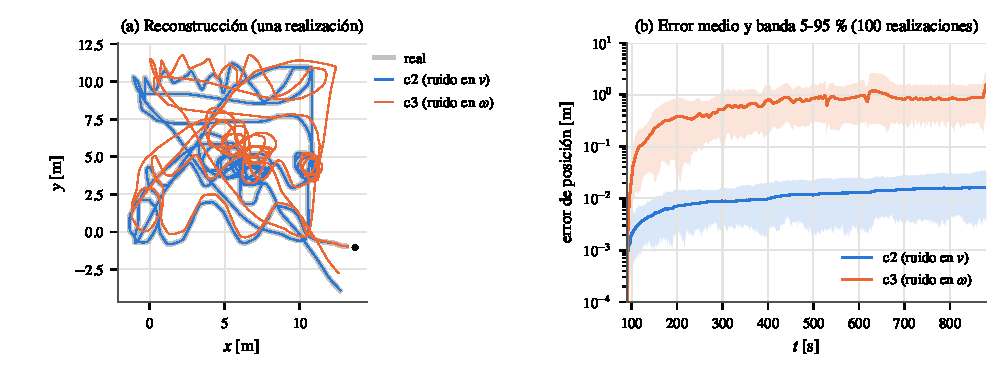
\includegraphics[width=\textwidth]{errores.pdf}
  \caption{(a) Trayectoria real y reconstruida en una realización de c2 y de c3 (punto negro: pose
  inicial). (b) Evolución del error de posición en escala logarítmica: media y banda entre los
  percentiles 5 y 95 de las \Nruns{} realizaciones. El caso c1 ($\sim10^{-13}$~m) queda fuera de escala.}
  \label{fig:errores}
\end{figure}

\textbf{c1, sin ruido.} El error es del orden de $10^{-13}$~m, es decir, error de redondeo de la
máquina: al integrar con la misma discretización con la que se derivaron $v$ y $\omega$, el proceso
es exactamente reversible.

\textbf{c2, ruido en $v$.} El error final medio es de \cDosFinal~m (\cDosPct\,\% del recorrido). El
ruido en $v$ solo altera la longitud de cada paso, no su dirección, y al ser de media nula los
errores se compensan parcialmente: crecen como un paseo aleatorio, lentamente
(fig.~\ref{fig:errores}b).

\textbf{c3, ruido en $\omega$.} El error final medio es de \cTresFinal~m, unas \ratioErr{} veces mayor
que en c2, con una dispersión muy grande entre realizaciones. El ruido en $\omega$ se integra en la
orientación, y un error de orientación se multiplica por toda la distancia recorrida después: la
trayectoria se deforma y gira (fig.~\ref{fig:errores}a). Además, $\sigma_\omega$ se calculó sobre
un $\overline{|\omega|}$ inflado por el ruido de cuantificación (apartado a), por lo que equivale a
algo más del 10\,\% del giro medio real.

\textbf{Conclusión.} En odometría la \textbf{orientación es la variable crítica}: un mismo error
relativo del 1\,\% produce un error de posición dos órdenes de magnitud mayor si afecta a $\omega$
que si afecta a $v$. Para una navegación prolongada conviene un giróscopo de calidad y corregir la
orientación periódicamente con una referencia absoluta (brújula, balizas, mapa o GPS) mediante
fusión sensorial.

% ------------------------------------------------------------------ Referencias
\begingroup
\small
\renewcommand{\refname}{Referencias}
\setlength{\itemsep}{0pt}
\begin{thebibliography}{9}
  \setlength{\itemsep}{1pt}
  \bibitem{gfg} GeeksforGeeks, ``Import Text Files Into Numpy Arrays -- Python'', 2026.
    \url{https://www.geeksforgeeks.org/python/import-text-files-into-numpy-arrays/}
  \bibitem{numpy} NumPy Developers, ``Structured arrays'', \emph{NumPy v2.5 Manual}.
    \url{https://numpy.org/doc/stable/user/basics.rec.html}
  \bibitem{matplotlib} The Matplotlib Development Team, ``Coding shortcuts'',
    \emph{Matplotlib 3.11.2 documentation}.
    \url{https://matplotlib.org/stable/tutorials/coding_shortcuts.html}
  \bibitem{upv} Universitat Politècnica de València, ``Rmóvil -- Cinemática -- Diferencial'',
    vídeo en YouTube. \url{https://www.youtube.com/watch?v=SirC01o7kx8}
  \bibitem{wiki} Wikipedia, ``Velocidad angular: velocidad angular en un movimiento plano general''.
    \url{https://es.wikipedia.org/wiki/Velocidad_angular\#Velocidad_angular_en_un_movimiento_plano_general}
\end{thebibliography}
\endgroup

\end{document}
